
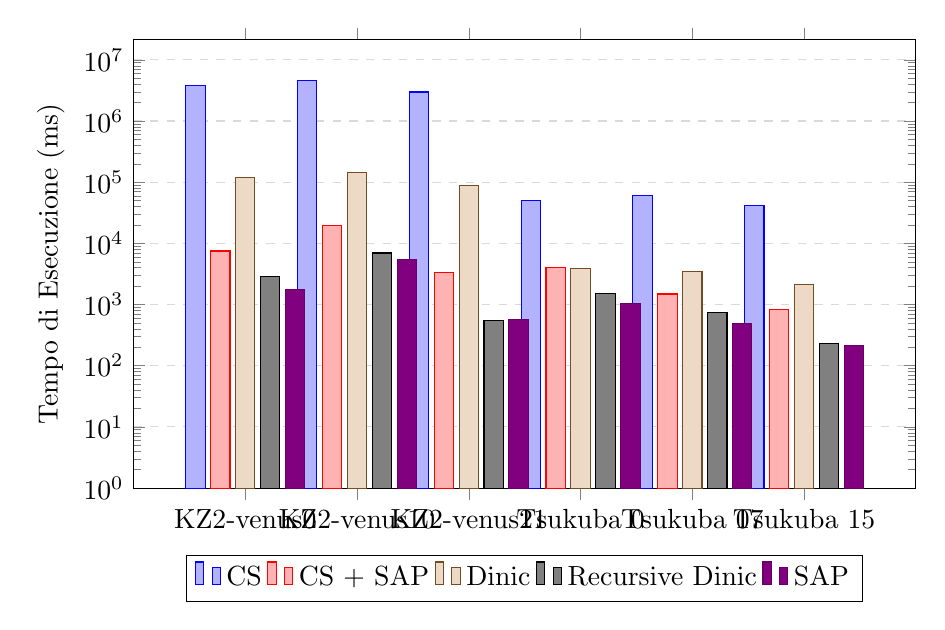
\begin{tikzpicture}
    \begin{semilogyaxis}[
        ybar,
        width=0.95\textwidth,
        height=0.6\textwidth,
        ylabel={Tempo di Esecuzione (ms)},
        symbolic x coords={KZ2-venus0,KZ2-venus10,KZ2-venus21,Tsukuba 0,Tsukuba 07,Tsukuba 15},
        xtick=data,
        point meta=y,
        legend style={at={(0.5,-0.15)}, anchor=north, legend columns=-1},
        ymajorgrids=true,
        grid style={dashed, gray!30},
        ymin=1,
        bar width=7pt,
        enlarge x limits=0.2
    ]
    \addplot coordinates {
        (KZ2-venus0, 3750051.34)
        (KZ2-venus10, 4597135.92)
        (KZ2-venus21, 2985202.47)
        (Tsukuba 0, 49953.22)
        (Tsukuba 07, 59929.96)
        (Tsukuba 15, 41804.45)
    };
    \addlegendentry{CS}
    \addplot coordinates {
        (KZ2-venus0, 7495.03)
        (KZ2-venus10, 19600.23)
        (KZ2-venus21, 3288.18)
        (Tsukuba 0, 4084.67)
        (Tsukuba 07, 1489.62)
        (Tsukuba 15, 817.88)
    };
    \addlegendentry{CS + SAP}
    \addplot coordinates {
        (KZ2-venus0, 118250.72)
        (KZ2-venus10, 143449.83)
        (KZ2-venus21, 89301.16)
        (Tsukuba 0, 3907.75)
        (Tsukuba 07, 3470.71)
        (Tsukuba 15, 2136.37)
    };
    \addlegendentry{Dinic}
    \addplot coordinates {
        (KZ2-venus0, 2867.96)
        (KZ2-venus10, 6963.97)
        (KZ2-venus21, 550.24)
        (Tsukuba 0, 1508.39)
        (Tsukuba 07, 753.65)
        (Tsukuba 15, 233.82)
    };
    \addlegendentry{Recursive Dinic}
    \addplot coordinates {
        (KZ2-venus0, 1773.21)
        (KZ2-venus10, 5451.56)
        (KZ2-venus21, 567.23)
        (Tsukuba 0, 1040.89)
        (Tsukuba 07, 490.83)
        (Tsukuba 15, 216.21)
    };
    \addlegendentry{SAP}

    \end{semilogyaxis}
\end{tikzpicture}
